\chapter{Architektur}

\section{Übersicht}

Um eine Drohne über einen Server in der Cloud steuern zu können, muss diese mit dem Internet verbunden werden. Dies ist nur über einen Proxy möglich, in diesem Fall ein Mobiltelefon. Das Mobiltelefon bietet andereseits auch eine Benutzeroberfläche um das Beladen und das Abfragen des Status der Drohne zu erleichtern. \\

\begin{figure}[h]
	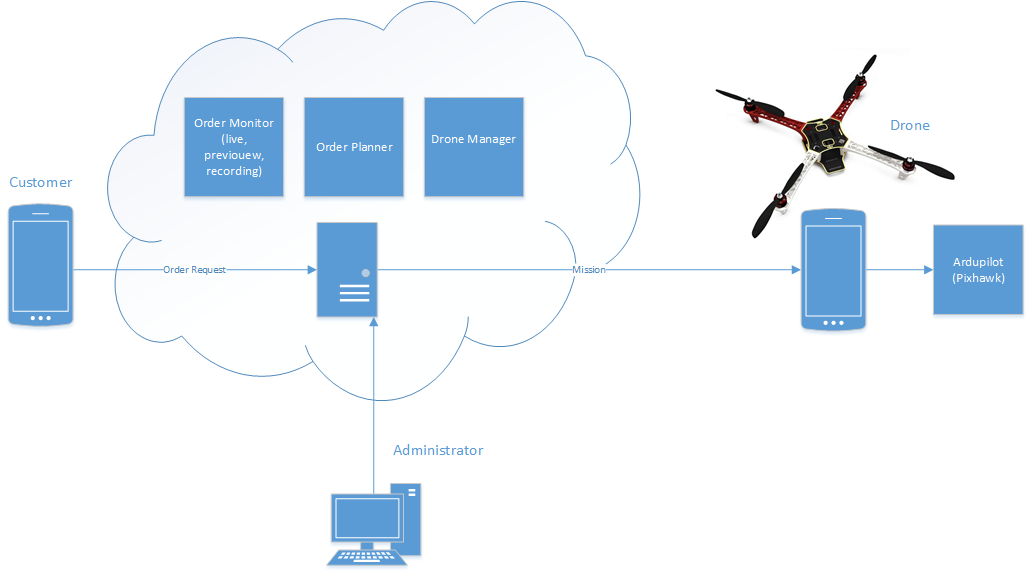
\includegraphics[width=1.0\textwidth]{images/Overview-Diagram.png}
	\caption{Übersicht der Project Helin Architektur }
	%\url{http://blog.placeit.net/free-avatar-pack/}}
	\label{fig:architecture-overview}
\end{figure}